\section{Outerplanar and Hamiltonian graphs}
Zoltán Lóránt Nagy showed that the conjecture of Goddard and Henning holds for
Hamiltonian graphs. For this, he characterized the $2$-coupon colorable
maximal outerplanar graphs.

\begin{definition}
   A graph is outerplanar if it has a planar drawing for which all vertices
   belong to the outer face. A maximal outerplanar graph is an outerplanar graph
   such that adding any edge results in a not outerplanar graphs.
\end{definition}
\begin{remark}
  Te outer face of a maximal outerplanar graph is a Hamiltonian cycle.
\end{remark}

In order to provide the mentioned characterization we need to introduce a few
notions first.
\begin{definition}
  Let $G$ be a maximal outerplanar graph of order $n \ge 3$. The $M(G)$ sun graph
  of $G$ is obtained by gluing a triangle to each edge of the outer face.
\end{definition}
\begin{remark}
  $M(G)$ is a maximal outerplanar graph with $2n$ vertices, from which $n$ has
  degree $2$.
\end{remark}
\begin{remark}
  If $G$ has an odd number of vertices, then $M(G)$ does not have two disjoint
  total dominating sets, as in a $2$-coupon coloring of $M(G)$, the vertices of
  $G$ must have alternating colors. The graph on figure $\ref{fig:sungraph}$ is
  the sun graph of the $BDE$ triangle.
\end{remark}
\begin{definition}
  A vertex $v$ of a maximal outerplanar graph is called a central vertex if the
  following $3$ conditions hold.
  \begin{enumerate}
    \item $deg(v) \ge 3$
    \item Every neighbor of $v$ has degree at least $3$
    \item For every $u, w$ neighbors of $v$ the length of the $uw$ path on the
    outer face not containing $v$ is divisible by $4$.
  \end{enumerate}
\end{definition}
\begin{claim}
  The outer face of a maximal outerplanar graph does not contain two consecutive
  central vertices.
\end{claim}
\begin{proof}
  Suppose there exists an $uv$ edge on the outer face such that $u$ and $v$ are
  central vertices. Because of the maximality of the graph there exists a $uvw$
  triangle. Index the vertices along the outer face form $v = v_1$ to $u = v_{n}$.
  Suppose $w = v_i$. From the centrality of $v$ follows that $i \equiv 2\
  (\textrm{mod}\ 4)$. On the other hand $u$ is also a central vertex, hence
  $i \equiv 1\ (\textrm{mod}\ 4)$.
\end{proof}
\begin{definition}
  A generalized sun graph is a maximal outerplanar graph of order
  $n \equiv 2\ (\textrm{mod}\ 4)$ such that the number of
  degree $2$ vertices plus the number of central vertices is $n/2$.
\end{definition}
\begin{remark}
  Every second vertex of the outer face in a generalized sun graph is either
  central or has degree $2$.
\end{remark}

The key characterization theorem is the following.

\begin{thm}\label{thm:outerplanar}
  Let $G$ be a maximal outerplanar graph. $G$ admits $2$ disjoint total dominating
  sets if and only if $G$ is not a generalized sun graph.
\end{thm}

For proving this theorem we need some observations about generalized sun graphs.
TODO

\begin{lemma}
  The outer face of a maximal outerplanar graph has a chord TODO
\end{lemma}

\begin{proof}[Proof of Theorem \ref{thm:outerplanar}]
  First we show that generalized sun graphs do not have $2$ disjoint total
  dominating sets. The proof goes by induction on the $n = 4k + 2$ number of vertices.

  For $k = 1$ there is only one generalized sun graph and it does not admit $2$
  disjoint total dominating sets. (Shown on figure \ref{fig:sungraph}.)

  Suppose $k \ge 2$ and $G$ is a generalized sun graph of order $4k + 2$. Index
  the vertices along the outer face from $v_1$ to $v_{4k + 2}$, such that every
  vertex with an odd index is central or has degree $2$. Let $c$ be a $2$-coloring of
  the graph. We show that $c$ cannot be a $2$-coupon coloring. The cardinality of the
  vertices implies that there must be two consecutive vertices $v_{2i}$ and $v_{2i + 2}$
  with the same color (say white). If $v_{2i}$ has only white neighbors, then this
  coloring is not a $2$-coupon coloring. So suppose $v_{2i}$ has a black neighbor
  $v_j$. In this case, $v_{2i}$ is a central vertex. The $v_{2i}v_j$ edge cuts the graph
  into two parts ($v_{2i}v_j$ is an edge in both graphs). Both of
  these graphs are generalized sun graphs, as $v_{2i}$ either remains a central
  vertex or become a vertex of degree $2$ in these smaller graphs, whereas other
  central vertices remain central vertices. By induction, the restriction of
  $c$ is not a $2$-coupon coloring in either of the smaller graphs. If there is
  a vertex $v_l$ with a monochromatic neighborhood in one of the smaller graphs
  and $l \neq 2i, l \neq j$, then $v_l$ has the same neighborhood in $G$, hence
  all its neighbors are from the same color class. $v_{2i}$ cannot violate the
  condition, as it was chosen in a way that it has both a black and a white neighbor
  in both graphs. Thus the only remaining case is when $v_j$ has a monochromatic
  neighborhood in both graphs. But in this case, all of its neighbors are from
  the same color class as $v_{2i}$, so it has a monochromatic neighborhood also
  in $G$.

  \vspace{0.4cm}

  Now we show that if a graph $G$ of order $n$ is not a generalized sun graph
  then it does have $2$ disjoint total dominating sets.

  If $n \equiv 0\ (\textrm{mod}\ 4)$, then it is easy to find a $2$-coupon coloring:
  color the vertices along the boundary of the outer face by repeating the pattern
  $BBWW$.

  If $n \equiv 1\ (\textrm{mod}\ 4)$, then the same coloring method works, if you
  start the coloring from the right vertex. By lemma \ref{lem:two_chord} there
  exists a chord $uv$ of length $2$. Alternating colors in pairs starting from $v$
  does the job.
  \begin{figure}[h]
    \centering
    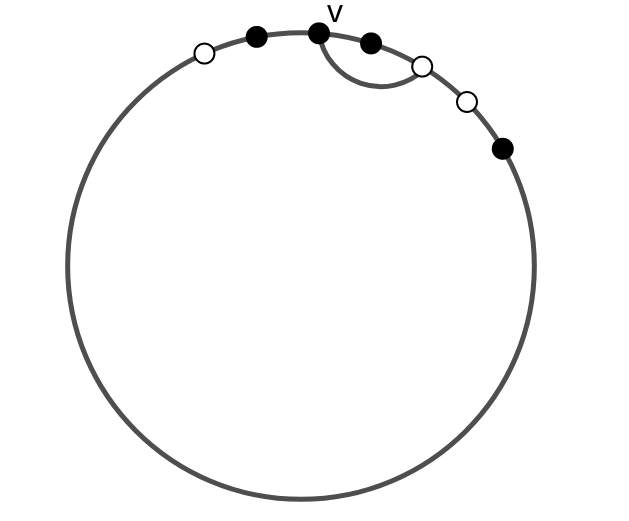
\includegraphics[width=50mm]{4k+1}
    \caption{Coloring an outerplanar graph of order $4k + 1$}
    \label{fig:4k+1}
  \end{figure}

  If $n \equiv 3\ (\textrm{mod}\ 4)$, then start the coloring from a vertex next
  to $v$.
  \begin{figure}[h]
    \centering
    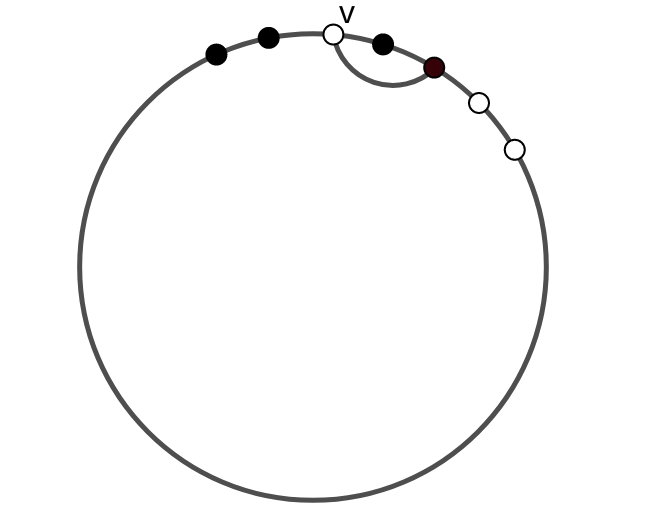
\includegraphics[width=50mm]{4k+3}
    \caption{Coloring an outerplanar graph of order $4k + 3$}
    \label{fig:4k+3}
  \end{figure}

  Suppose $n \equiv 2\ (\textrm{mod}\ 4)$. We show that if $G$ does not have $2$
  disjoint total dominating sets, then it is a generalized sun graph.

  TODO
\end{proof}

\begin{remark}
  With a slight modification of the proof it can be shown that the vertices of a
  generalized sun graph cannot be colored in a way that every degree $2$ or central
  vertex has neighbors from both color classes.
\end{remark}

\begin{thm}
  Every triangulated graph with a Hamiltonian circle admits $2$ disjoint
  dominating sets.
\end{thm}
\begin{proof}
  Let $G$ be a triangulated Hamiltonian graph and let $n$ denote the number of
  vertices in $G$.

  TODO
\end{proof}

\section{Graphs without low-degree vertices}
TODO (Find the related article)

\section{A result using hypergraphs}
TODO

\section{Barnette's conjecture}
\begin{conj}
  Every 3-connected cubic planar bipartite graph is Hamiltonian.
\end{conj}
